%\documentclass[a4paper]{article}
%\usepackage[margin=2cm]{geometry} % отступ сбоку
%\usepackage[utf8x]{inputenc} % поддержка utf8
%\usepackage[english,russian]{babel} % поддержка переностов слов
%\usepackage{ctable} % для толстых линий с specialrule
%\usepackage{graphicx} % для вставки картинок
%\usepackage{calc} % для рассчётов внутри squarecells
%\usepackage{array} % для рассчётов внутри squarecells
%\usepackage{tabularx} % таблички
%\usepackage{rotating} % поворот квадратика 
%\usepackage{amssymb} % символ квадратика
%\usepackage{setspace} % для регулировки межстрочного интервала через spacing
%\usepackage{blindtext}

\pagenumbering{gobble}
%\sloppy % выравнивание по ширине (надо-ли?)

% открытие секции squarecells
\newlength\celldim
\newlength\fontheight
\newlength\extraheight
\newcounter{sqcolumns}

\newcolumntype{B}{!{\vrule width .2em}}
\newcolumntype{S}{
    @{}
    >{\centering \rule[-0.5\extraheight]{0pt}{\fontheight + \extraheight}%
    \begin{minipage}{\celldim}\centering}
    p{\celldim}
    <{\end{minipage}} 
    @{}
}
\newcolumntype{T}{ @{} >{\centering} p{\celldim} @{} }

\newenvironment{squarecells}[1]
    {
        \setlength\celldim{1.7em}
        \settoheight\fontheight{е}
        \setlength\extraheight{\celldim - \fontheight}
        \setcounter{sqcolumns}{#1 - 2}
        \begin{tabular}{BS|*{\value{sqcolumns}}{T|}TB}\specialrule{.2em}{.1em}{.1em}
    }
    {
        \specialrule{.2em}{.1em}{.1em}\end{tabular}
    }

\newcommand\nl{\tabularnewline\hline}
% закрытие секции squarecells



\begin{document}
    \begin{tabular}{p{0.3\textwidth}p{0.6\textwidth}}
        \vspace{87}
        \textbf{Ф617.}
        \itshape Газетный текст фотографируется аппаратом «Зенит» c объективом, имеющим фокусное расстояние 50мм. дважды:\newline % newline чтоб не натравить табоицу закрытие колонки
        1) c наименьшего допустимого для этого объектива a=0,5 м; \newline
        2) после присоединения объектива к камере через удлинительное кольцо высотой h = 25 мм (таeже с минимально возможного расстояния). Найдите отношение размеров изображений, полученных на фотомплёнке в этих двух случаях.\newline 
        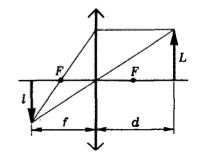
\includegraphics[width=0.29\textwidth]{image} 

        &

        \begin{center}
            Решая совместо уравнения (1) и (2), находим
        \end{center}
        \begin{center}
            $l_{1} = l \sqrt[3]{2}, d_{1} = d \sqrt[3]{4}$.
        \end{center}
        \begin{flushright}
            \itshapeИ. Слободецкий % использую itshape из-за несовместимости textit и flushright
        \end{flushright}
        \hspace{3}
        \begin{rotate}{55}
            $\blacksquare$
        \end{rotate}

        Для решения задачи воспользуемся формулой линзы
        \begin{center}
            $\frac{1}{d} + \frac{1}{f} = \frac{1}{F}$,
        \end{center}
        где d - рассотяние от фотографируемого предмета до объектива, f - расстояние от объектива до изображения, F - фокусное расстояние объектива (см. рисунок).\newline
        \null\quadПри фотографировании текста в первом случае (без удлинительного кольца) $d_{1}=a$, и резкое изображение получается на расстоянии % используем \null т.к quad не захватывается, если стоит в начале строки
        \begin{center}
            $f_{1}=\frac{aF}{a-F}$.
        \end{center}
        Линейный размер изображения в этом случае равен (см. рисунок).
        \begin{center}
            $l_{1} = L\frac{f_{1}}{a} = L\frac{F}{a-F}$.
        \end{center}
        \quad При присоединении объектива к камере через удлинительное колтцо высотой h резкое изображение текста получается на расстоянии
        \begin{center}
            $f_{2}=f_{1}+h=\frac{aF}{a-F}+h$
        \end{center}
        от объектива. Минимально возможное расстояние от объектива, на котором может находиться при фотографировании текст, в этом случае равно
        \begin{center}
            $d_{1}=\frac{f_{2}F}{f_{2}-F}=\frac{(aF+h(a-F))F}{F^{2}+h(a-F)}$.
        \end{center}
        Размер изображения в этом случае
        \begin{center}
            $l_{2}=L\frac{f_{2}}{d_{2}}=L(\frac{F}{a-F}+\frac{h}{F})$.
        \end{center}
        \quad Таким обрахом, отношение размеров изображений, полученных на фотопленке в двух случаях равно
        \begin{center}
            $\frac{l_{2}}{l_{1}}=\frac{h(a-F}{F^{2}}+l=5,5$.
        \end{center}
        \begin{flushright}
            \itshapeВ. Дерябкин
        \end{flushright}
        \\
    \end{tabular}

    \hrule

    \begin{tabular}{p{0.3\textwidth}>{\Centering}p{0.3\textwidth}p{0.3\textwidth}}
        \vspace{22}
        \begin{spacing}{1.125} % ставим большой межстрочный интервал
            \huge{\textbf{Неоконченная}}
            \huge{\textbf{криптограмма}}
        \end{spacing}
        \smallПеред вами криптограмма, которую можно прочесь с помощью некоторой решетки (что это такое, вы узнаете, прочитав статью «Самосовмещения квадрата и тайнопись» на с. 31), накладывая её поcледовательно
        
        &
    
        \vspace{0}
        \begin{center}
            \begin{squarecells}{8}
                е & м & ы & в & л & е & о & р \nl
                г & б & н & а & и & о & я & л \nl
                ч &   & о & о & в & л &   & е \nl
                е & ь &   & м &   & в & а & ш \nl
                  & г & р & е & х & в &   & о \nl
                и & о &   & л &   & о & о & м \nl
                в & е & е & д & б & а &   & г \nl
                р &   & а &   & о &   & ж & б \tabularnewline
            \end{squarecells}
        \end{center}
        
        &
        
        \vspace{23}
        4 раза (каждый раз - с поворотом на 90\degree). В зашифрованном в ней сообщении букв меньшеЮ чем клеток квадрата, так что некоторые его оказываются «лишними». Здесь все «лишние» клетеи оставлены пустыми.\newline
        \null\quad Расшифруйте зашифрованное сообщение.
        \begin{flushright}
            \itshape Э. Рекстин
        \end{flushright}
        \\
    \end{tabular}
    \vfill
    \begin{flushright}
        \textbf{29}
    \end{flushright}
\end{document}